\documentclass[crop, tikz,convert=pdf2svg]{standalone}
\usetikzlibrary{calc,positioning,fit,backgrounds,shapes.symbols}
\begin{document}
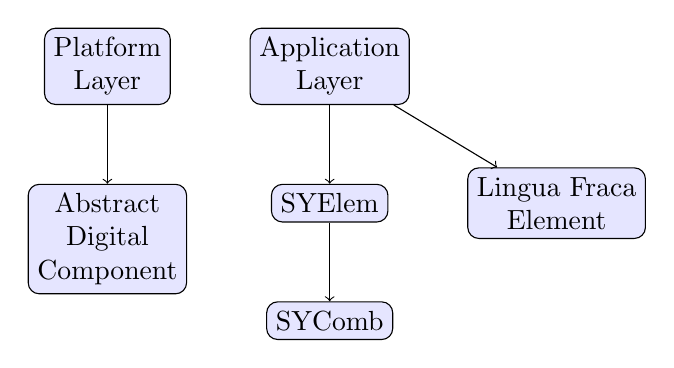
\begin{tikzpicture}[
    trait/.style={rounded corners, fill=blue!10, draw=black, align={center}}
  ]
  \node[trait] (applayer) {Application\\ Layer};
  \node[trait, below=of applayer] (syelem) {SYElem};
  \node[trait, below=of syelem] (sycomb) {SYComb};
  \node[trait, right=of syelem] (lfelem) {Lingua Fraca\\ Element};
  \node[trait, left=of applayer] (platlayer) {Platform\\ Layer};
  \node[trait, below=of platlayer] (absdigcomp) {Abstract\\ Digital\\ Component};

  \draw[->] (applayer) -- (syelem);
  \draw[->] (syelem) -- (sycomb);
  \draw[->] (applayer) -- (lfelem);
  \draw[->] (platlayer) -- (absdigcomp);
\end{tikzpicture}
\end{document}